\documentclass[a4paper]{article}
\usepackage[english,spanish]{babel}
\usepackage[utf8]{inputenc}
\usepackage[T1]{fontenc}
\usepackage{verse}
\usepackage[noend]{algpseudocode}
\usepackage{listings}
%% Sets page size and margins
\usepackage[a4paper,top=3cm,bottom=3cm,left=3cm,right=3cm,marginparwidth=1.75cm]{geometry}
%% Useful packages
\usepackage{amssymb,amsmath,amsthm,amsfonts}
\usepackage{graphicx}
\usepackage[colorinlistoftodos]{todonotes}
\usepackage[colorlinks=true, allcolors=blue]{hyperref}

\newcommand{\verso}[1] {
\settowidth{\versewidth}{123456789012345678901234567890}%
\begin{minipage}[t]{\dimexpr\versewidth+1pt\relax}
\begin{verse}[\versewidth]
{\fontfamily{qzc}\selectfont\large
  #1
}
\end{verse}
\end{minipage}\bigskip
}

\title{Trabajo Práctico 1 (Los monos de Shakespeare)}
\author{Sebastián Cherny}



\begin{document}
\maketitle

1)\\
Para simular lo que va escribiendo el mono, agrego una letra a la palabra que viene escribiendo, simulando la escritura de una letra con una extracción al azar del conjunto de letras (en este caso ('A', 'B'), pero podría generalizarse), donde cada letra tiene la misma probabilidad (función sample).

El código lo que hace es primero escribir la misma cantidad de letras que tiene la palabra dada, y a partir de ahí, mientras no tenga la palabra deseada, descarto la primera letra, y agrego una al final, en vez de simplemente agregar una letra y preguntar si está la palabra deseada en la palabra total, ya que si hasta ahora no estaba, todo lo que importa es ver si está al agregarse la última letra.
La función 'substr' podría ser lenta pero como después queremos buscar una palabra en otra, si lo hacemos linealmente la complejidad termina siendo la misma.

Algo interesante podría ser pensar una lógica parecida al llamado algoritmo Z para saber de una manera eficiente qué pasa cuando muevo todos los caracteres hacia la izquierda (descartando el primero), es decir cuál es el prefijo más largo que queda matcheada a la palabra deseada.

2)\\
Salida de una corrida:
\\
Para escribir la palabra AA se necesita en promedio 6.058\\
Para escribir la palabra AB se necesita en promedio 4.06\\
Para escribir la palabra AAA se necesita en promedio 14.434\\
Para escribir la palabra AAB se necesita en promedio 7.918\\
Para escribir la palabra ABA se necesita en promedio 9.854\\
Para escribir la palabra BABA se necesita en promedio 18.815\\
Para escribir la palabra BABAB se necesita en promedio 42.926\\


Se puede ver que el tiempo esperado no depende sólo de la longitud de la palabra, ya que por ejemplo el tiempo promedio para AAA es cerca del doble del tiempo promedio para AAB. En este ejemplo se ve clara la razón. Si el mono está escribiendo, con el objetivo de escribir AAA, al tipear una letra B, todo el tiempo que pasó hasta ahora fue en vano, y estaría volviendo a empezar.\\
Sin embargo, si el objetivo es AAB, si el mono tipea AAA, el error en la tercera letra no afecta tanto ya que seguimos con las primeras dos letras "matcheadas" a nuestro objetivo, sigue faltándonos una letra. De hecho, una vez que el mono tipea dos letras A juntas, a partir de ahí terminará con la primera aparición de una B.\\
Para este caso, podemos ver estas particularidades: La probabilidad de escribir ambas palabras en exactamente 3 caracteres es igual, pero la cantidad de distintas secuencias de 4 caracteres que generan cada palabra son:\\
Para AAA: BAAA\\
Para AAB: BAAB, AAAB\\
\\
Creo que el tiempo estimado tiene que ver, además de un poco con la longitud de la palabra (es mucho más probable tipear $3$ letras $A$ consecutivas en algún momento que $5$), con la longitud máxima de prefijo que también es sufijo, por lo mencionado en el caso de AAA y AAB, que si bien ambos empiezan con AA y tienen $3$ letras, el tiempo estimado de una es casi el doble que el de la otra.

3)\\
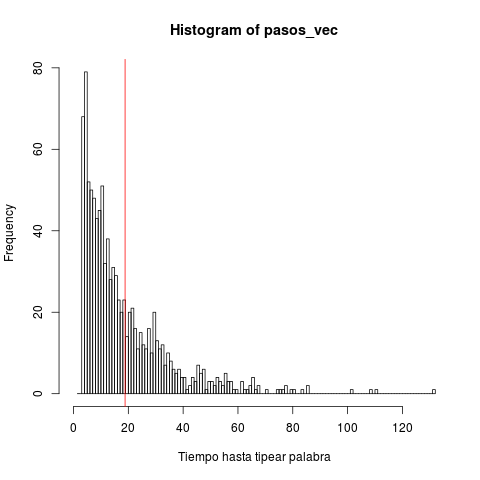
\includegraphics[width=12cm,height=9cm,keepaspectratio]{histograma_BABA.png}
\\
Se puede ver en el gráfico de barras, que la probabilidad se asimila a una exponencial, pero podemos ser más genéricos y decir que la familia del tiempo esperado parecería ser una distribución Gamma.

Algo que se me ocurre para pensar que la probabilidad disminuye es pensar que para escribir una palabra de $C$ caracteres en exactamente $L$ caracteres, los últimos $C$ siempre tendrán que coincidir, por lo que para pegarle justo a cada letra de la secuencia en el orden correcto ya tengo la misma probabilidad que para escribirla en los primeros $C$ caracteres. Y si pensamos en 'cuántas secuencias de $L$ caracteres terminan con nuestra palabra y no la contienen antes del final', tenemos que descartar todas las secuencias que contienen a la palabra anteriormente del total de secuencias posibles de $L$ letras, cuando mirando sólo los primeros $C$ caracteres no tenemos que descartar nada.

\end{document}